\documentclass[11pt, a4paper]{article}
\usepackage[a4paper, margin=1in]{geometry}


\usepackage{adjustbox}
\usepackage{mathtools}
\usepackage{amsmath}
\usepackage{amssymb}
\usepackage{amsthm}

\usepackage{pgfplots}
\usepackage{listings}
\usepackage{color}
\usepackage{tikz}

\usepackage{textcomp}
\usepackage{soul}

\usepackage[hidelinks]{hyperref}
\pgfplotsset{width=7.5cm,compat=1.12}
\usepgfplotslibrary{fillbetween}
\usepackage[makeroom]{cancel}
\title{\bf{Homework \textnumero 2}}
\author{Author: David Oniani
\\
\ \ \ Instructor: Dr. Eric Westlund}
\date{February 11, 2019}

\usepackage{listings}
\usepackage{color}

%%%%%%%%%%%%%%% S E T S %%%%%%%%%%%%%%%
\newcommand{\nats}{\mathbb{N}}
\newcommand{\ints}{\mathbb{Z}}
\newcommand{\rats}{\mathbb{Q}}
\newcommand{\reals}{\mathbb{R}}
\newcommand{\irrats}{\mathbb{I}}

\newcommand{\pnats}{\mathbb{N}^+}
\newcommand{\pints}{\mathbb{Z}^+}
\newcommand{\prats}{\mathbb{Q}^+}
\newcommand{\preals}{\mathbb{R}^+}
\newcommand{\nreals}{\mathbb{R}^-}

\newcommand{\nints}{\mathbb{Z}^-}
\newcommand{\nrats}{\mathbb{Q}^-}
%%%%%%%%%%%%%%%%%%%%%%%%%%%%%%%%%%%%%%%

% Calligraphy
\newcommand\und[1]{\underline{\smash{#1}}}

% Operators
\DeclarePairedDelimiter\abs{\lvert}{\rvert}
\DeclarePairedDelimiter\ceil{\lceil}{\rceil}
\DeclarePairedDelimiter\floor{\lfloor}{\rfloor}

% Other
\newcommand{\rarr}{\rightarrow}

\definecolor{dkgreen}{rgb}{0,0.6,0}
\definecolor{gray}{rgb}{0.5,0.5,0.5}
\definecolor{mauve}{rgb}{0.58,0,0.82}
\definecolor{backcolour}{rgb}{0.95,0.95,0.92}

\lstset{
backgroundcolor=\color{backcolour},
aboveskip=3mm,
belowskip=3mm,
showstringspaces=false,
columns=flexible,
basicstyle={\small\ttfamily},
numbers=left,
numberstyle=\normalsize\color{gray},
keywordstyle=\color{blue},
commentstyle=\color{dkgreen},
stringstyle=\color{mauve},
breaklines=true,
breakatwhitespace=true,
tabsize=4
}


\begin{document}
\maketitle
\begin{itemize}
\item[2.4]
Well, since $\$270, 900$ is nowhere near $\$340, 300$, it means that the distribution
is not symmetric. Now, since the distribution is not symmetric, it means that it is skewed.
In this case, it would be a right-skewed distribution and therefore the mean will
be greater than the median. Finally, we have that the mean is $\$340, 300$ and the median is $\$270, 900$.

\item[]

\item[2.5]
The mean is the sum of CO$_2$ emission for all states divided by 50. After a tedious
calculation, one will get that the mean is approximately $4.606$. The median, in this case,
will be the $19^{\text{th}}$ element in the list of this data in the sorted order.
The data in the sorted order looks like this:

\begin{center}
\begin{verbatim}
data = [0.0746, 0.1113, 0.1522, 0.1732, 0.3038,
        0.3109, 0.3716, 0.4932, 0.4941, 0.8731,
        0.9321, 1.5994, 1.6295, 1.6662, 1.7281,
        1.8032, 2.1503, 2.6228, 3.3315, 3.7034,
        3.7636, 4.131, 4.4469, 4.471, 5.5554,
        5.8535, 6.1949, 6.6449, 6.7177, 7.6765,
        7.9251, 8.3086, 9.1148, 9.1857, 9.2041,
        11.4869, 12.2255, 14.6261, 17.5642]
\end{verbatim}
\end{center}

Then it is easy to see that the $19^{\text{th}}$ element is $3.3315$
and therefore the median is $3.3315$.

Here is the histogram for the given data:
\begin{center}
    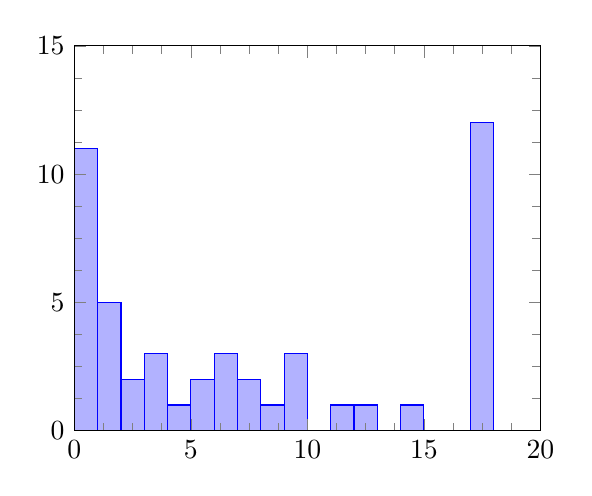
\begin{tikzpicture}
        \begin{axis}[
            ymin=0, ymax=15,
            xmin=0, xmax=20,
            minor y tick num = 3,
            minor x tick num = 3,
            area style,
            ]
        \addplot+[ybar interval, mark=no] plot coordinates { (0, 11) (1, 5) (2, 2) (3, 3) (4, 1) (5, 2) (6, 3) (7, 2) (8, 1) (9, 3) (10, 0) (11, 1) (12, 1) (13, 0) (14, 1) (15, 0) (16, 0) (17, 12) (18, 0) };
        \end{axis}
    \end{tikzpicture}
\end{center}

The mean is larger than the distribution since we have an outlier (the tallest bar in the end)
which distorts the actual picture (the median, however, is resistant).

\newpage

\item[2.6]
\begin{itemize}
\item[(a)]
The stemplot for the data of defensive linemen is
\item[]
\item[]

\begin{center}
\begin{tabular}{r | *{120}{c}}
    24 & 2\\
    25 & 2 & 4\\
    26 & 0\\
    27 & 4\\
    28 & \\
    29 & 7\\
    30 & 0 & 3\\
    31 & 1\\
    32 & 3
\end{tabular}
\end{center}

\item[]
\item[]
\textbf{\und{Five-number summary}}\\\\
Minimum is $242$.\\\\
$Q_1$ is $254$.\\\\
Median is $\dfrac{274 + 297}{2} = 285.5$.\\\\
$Q_3$ is $303$.\\\\
Maximum is $323$.

\item[]

\item[(b)]
The stemplot for the data of offensive linemen is
\item[]
\item[]
\begin{center}
    \begin{tabular}{r | *{120}{c}}
        29 & 8\\
        30 & 1 & 5\\
        31 & 0 & 5 & 8\\
        32 & 0 & 1\\
        33 & 2
    \end{tabular}
\end{center}

\item[]
\item[]
\textbf{\und{Five-number summary}}\\\\
Minimum is $298$.\\\\
$Q_1$ is $\dfrac{301 + 305}{2} = 303$.\\\\
Median is $315$.\\\\
$Q_3$ is $\dfrac{320 + 321}{2} = 320.5$.\\\\
Maximum is $332$.

\item[]

\item[(c)]
The stemplot for offensive linemen is symmetric and has
not outliers. The stemplot for defensive linemen is almost
symmetric and also does not have any outliers. The group
of offensive linemen are heavier since its datapoints have
higher values
\end{itemize}

\item[]
\item[]

\item[7.]
\textbf{\und{Five-number summary}}\\\\
Minimum is $11$.\\\\
$Q_1$ is $18$.\\\\
Median is $21$.\\\\
$Q_3$ is $26$.\\\\
Maximum is $51$.

\end{itemize}
\end{document}
